\begin{figure}[htbp]
\centering
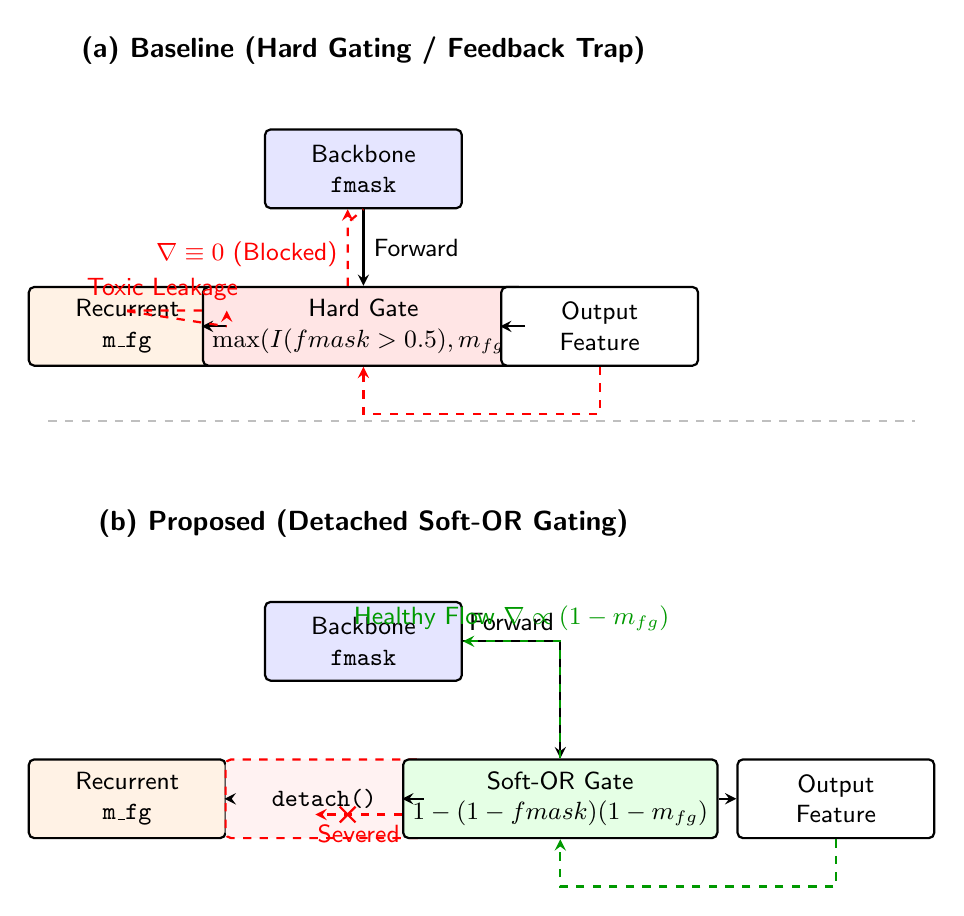
\begin{tikzpicture}[
    >=stealth,
    node distance=1.5cm and 2cm,
    font=\sffamily\small,
    box/.style={rectangle, draw=black, thick, minimum width=2.5cm, minimum height=1cm, align=center, fill=white, rounded corners=2pt},
    gate/.style={rectangle, draw=black, thick, minimum width=2.5cm, minimum height=1cm, align=center, fill=gray!10, rounded corners=2pt},
    detach/.style={rectangle, draw=red, thick, dashed, minimum width=2.5cm, minimum height=1cm, align=center, fill=red!5, rounded corners=2pt},
    fwd/.style={->, thick, solid, draw=black},
    bwd_red/.style={->, thick, dashed, draw=red},
    bwd_green/.style={->, thick, dashed, draw=green!60!black},
    title/.style={font=\sffamily\bfseries\normalsize}
]

% =========================================================
% Panel (a): Standard MixPool (Feedback Trap)
% =========================================================
\node[title] (title_a) at (0, 3.5) {(a) Baseline (Hard Gating / Feedback Trap)};

% Nodes for (a)
\node[box, fill=blue!10] (fmask_a) at (0, 2) {Backbone \\ \texttt{fmask}};
\node[box, fill=orange!10] (m_a) at (-3, 0) {Recurrent \\ \texttt{m\_fg}};
\node[gate, fill=red!10] (gate_a) at (0, 0) {Hard Gate \\ $\max(\mathbb{I}(\text{fmask}>0.5), m_{\text{fg}})$};
\node[box] (out_a) at (3, 0) {Output \\ Feature};

% Forward Pass (a)
\draw[fwd] (fmask_a) -- (gate_a) node[midway, right] {Forward};
\draw[fwd] (m_a) -- (gate_a);
\draw[fwd] (gate_a) -- (out_a);

% Backward Pass (Gradient) (a)
% Gradient from Output to Gate
\draw[bwd_red] (out_a.south) -- +(0,-0.6) -| (gate_a.south);
% Blocked gradient to fmask
\draw[bwd_red] (gate_a.north) ++(-0.2,0) -- ++(0, 0.8) node[midway, left, text=red] {$\nabla \equiv 0$ (Blocked)} -- (fmask_a.south |- fmask_a.south) ++(-0.2,0);
% Toxic gradient to recurrent mask
\draw[bwd_red] (gate_a.west) ++(0, 0.2) -- ++(-1, 0) node[midway, above, text=red] {Toxic Leakage} -- (m_a.east |- m_a.east) ++(0, 0.2);


% =========================================================
% Panel (b): Proposed Detached Soft-OR
% =========================================================
\node[title] (title_b) at (0, -2.5) {(b) Proposed (Detached Soft-OR Gating)};

% Nodes for (b)
\node[box, fill=blue!10] (fmask_b) at (0, -4) {Backbone \\ \texttt{fmask}};
\node[box, fill=orange!10] (m_b) at (-3, -6) {Recurrent \\ \texttt{m\_fg}};
\node[detach] (detach_b) at (-0.5, -6) {\texttt{detach()}};
\node[gate, fill=green!10] (gate_b) at (2.5, -6) {Soft-OR Gate \\ $1 - (1-\text{fmask})(1-m_{\text{fg}})$};
\node[box] (out_b) at (6, -6) {Output \\ Feature};

% Forward Pass (b)
\draw[fwd] (fmask_b) -| (gate_b) node[pos=0.25, above] {Forward};
\draw[fwd] (m_b) -- (detach_b);
\draw[fwd] (detach_b) -- (gate_b);
\draw[fwd] (gate_b) -- (out_b);

% Backward Pass (Gradient) (b)
% Gradient from Output to Gate
\draw[bwd_green] (out_b.south) -- +(0,-0.6) -| (gate_b.south);
% Healthy gradient to fmask
\draw[bwd_green] (gate_b.north) ++(0,0) |- (fmask_b.east) node[pos=0.75, above, text=green!60!black] {Healthy Flow $\nabla \propto (1 - m_{\text{fg}})$};
% Severed gradient at detach
\draw[bwd_red] (gate_b.west) ++(0, -0.2) -- ++(-1.1, 0) node[midway, below, text=red] {Severed};
% Cross mark to show detachment
\draw[red, thick] (-0.3, -6.1) -- (-0.1, -6.3);
\draw[red, thick] (-0.3, -6.3) -- (-0.1, -6.1);

% Draw separator line
\draw[dashed, gray!50, thick] (-4, -1.2) -- (7, -1.2);

\end{tikzpicture}
\caption{Visual comparison of the (a) Standard Feedback Trap and (b) Proposed Detached Soft-OR mechanism. Solid black arrows denote the forward representation pass. Dashed arrows trace the backward gradient path. In (a), the hard binary gate paralyzes gradient flow to the backbone (Red dashed, $\nabla \equiv 0$) while leaking toxic gradients back into the recurrent loop. In (b), our proposed \texttt{detach()} barrier structurally severs the recurrent error loop, while the continuous Soft-OR operator restores a healthy, uncertainty-guided gradient flow (Green dashed, $\nabla \propto (1-m_{\text{fg}})$) directly to the internal attention branch.}
\label{fig:architecture_tikz}
\end{figure}
